% Nature Machine Intelligence Format
% FNO-RC: Fourier Neural Operator with Continuous Fourier Transform Residual Correction
\documentclass[11pt]{article}

% Essential packages
\usepackage[margin=1in]{geometry}
\usepackage{times}
\usepackage{amsmath, amssymb, amsthm}
\usepackage{graphicx}
\usepackage{booktabs}
\usepackage{subcaption}
\usepackage{multirow}
\usepackage{siunitx}
\usepackage{natbib}
\usepackage{hyperref}
\usepackage{tikz}
\usetikzlibrary{shapes,arrows,positioning,calc}
\hypersetup{colorlinks=true, linkcolor=blue, citecolor=blue, urlcolor=blue}

% Math commands
\newcommand{\R}{\mathbb{R}}
\newcommand{\C}{\mathbb{C}}
\newcommand{\F}{\mathcal{F}}
\newcommand{\G}{\mathcal{G}}
\newcommand{\K}{\mathcal{K}}
\newcommand{\norm}[1]{\left\|#1\right\|}

% Theorem environments
\newtheorem{theorem}{Theorem}
\newtheorem{proposition}{Proposition}

\title{\textbf{Fourier Neural Operator with Continuous Fourier Transform Residual Correction for Partial Differential Equation Solving}}

\author{
    Taiqian Liu$^{1}$, Lijun Liu$^{1,*}$ \\
    \\
    $^{1}$School of Informatics, Xiamen University, Xiamen, China \\
    $^{*}$Corresponding author: lijun.liu@xmu.edu.cn
}

\date{}

\begin{document}

\maketitle

\begin{abstract}
Fourier Neural Operators (FNOs) have revolutionized PDE solving by learning solution operators through spectral parameterization. Yet discrete Fourier transforms impose critical bottlenecks: aliasing artifacts from finite sampling, artificial periodicity that conflicts with physical boundaries, and catastrophic error accumulation during long-term predictions. Here we present FNO-RC, a dual-path architecture augmenting standard FNO with Continuous Fourier Transform residual correction. Our approach leverages piecewise Chebyshev expansions to capture high-frequency spectral content that FFT fundamentally cannot represent—achieving this through strategic shallow-layer activation and targeted regularization that prevents instability. Across three benchmark problems, FNO-RC delivers striking gains: while the 1D Burgers equation sees modest 3.01\% improvement, 2D Navier-Stokes accuracy jumps by \textbf{73.68\%}, and high-Reynolds turbulence ($Re=10^4$) improves 43.76\%. Cross-resolution tests, 100-step autoregressive rollouts, and spectral diagnostics consistently validate our method. This work reveals how hybridizing continuous and discrete spectral representations can overcome long-standing limitations in neural PDE solvers.
\end{abstract}

\section{Introduction}

Physical systems—from turbulent flows to quantum dynamics—evolve according to partial differential equations. While traditional numerical solvers remain the gold standard for accuracy, they buckle under dimensionality curses and demand prohibitive computational budgets at high resolutions. Neural operators \citep{kovachki2021neural,lu2021learning} offer an intriguing alternative: rather than approximating functions pointwise, they learn mappings between infinite-dimensional function spaces. Among these, Fourier Neural Operators (FNOs) \citep{Li2020FNO} stand out. By parameterizing integral kernels in Fourier space and exploiting the convolution theorem, FNOs achieve resolution-invariant learning—sometimes accelerating simulations by orders of magnitude.

However, FNO's reliance on discrete Fourier transforms creates deep-rooted pathologies. Finite sampling triggers spectral aliasing; periodic boundary assumptions clash with real-world physics; mode truncation obliterates high-frequency features essential for shocks and vortices. Perhaps most insidious: small spectral biases compound exponentially during autoregressive prediction, causing catastrophic divergence in chaotic systems.

Enter \textbf{FNO-RC}—our dual-path architecture that marries standard FNO with a Continuous Fourier Transform residual branch. The central observation? CFT handles discontinuities through conformal mapping and Chebyshev polynomial discretization \citep{barnett2010conformal}, achieving exponential convergence where DFT falters algebraically. We activate this correction strategically: shallow layers only, time-dependent but spatially broadcast, rigorously regularized against instability.

\textbf{Contributions.} Beyond proposing the dual-path architecture, we establish its mathematical foundations and demonstrate breakthrough empirical gains: 73.68\% improvement on 2D Navier-Stokes, 43.76\% on 3D high-Reynolds turbulence. Cross-resolution tests, 100-step rollouts, and spectral diagnostics paint a consistent picture of success.

\section{Background and Related Work}

\textbf{Neural Operators.} Learning operators—not just functions—marks a conceptual leap \citep{kovachki2021neural,azizzadenesheli2024neural}. Where traditional networks map finite vectors, neural operators target maps $\G: \mathcal{U} \rightarrow \mathcal{V}$ between infinite-dimensional spaces. DeepONet \citep{lu2021learning,wang2021learning} pioneered this via branch-trunk decomposition, though its point-wise evaluation limits efficiency. Graph approaches \citep{li2020multipole,li2020neural} excel on irregular meshes but struggle with global interactions.

FNO \citep{Li2020FNO} changed the game: Fourier-space kernel parameterization enables $O(N \log N)$ global convolutions. Yet its variants reveal tensions in the field. Factorized FNO \citep{tran2021factorized} trades accuracy for speed through low-rank decomposition—a compromise that hurts turbulent flows. Geo-FNO \citep{li2023geometry} handles curved geometries elegantly but at substantial implementation cost. U-FNO \citep{wen2022u} imports multi-scale U-Net ideas, though whether spatial hierarchy truly benefits spectral methods remains debatable. AFNO \citep{guibas2021adaptive,pathak2022fourcastnet} adds attention—impressively scaling to weather forecasting, but do we really need such complexity for PDE operators? Physics-Informed FNO \citep{li2021physics} enforces constraints as soft penalties, begging the question: how hard should we bake in physics versus letting data speak?

\textbf{Spectral Methods.} Classical spectral collocation \citep{boyd2001chebyshev,trefethen2019approximation} achieves exponential convergence for smooth solutions via orthogonal polynomials. The catch? Gibbs oscillations demolish accuracy near discontinuities. PINNs \citep{raissi2019physics,karniadakis2021physics} merge neural networks with residuals—conceptually appealing, but high-frequency features and loss-weight tuning remain thorny in practice.

\textbf{Continuous Fourier Transform.} Barnett and Greengard's conformal approach \citep{barnett2010conformal} sidesteps Gibbs artifacts through complex-plane deformation and Chebyshev discretization. We're the first to harness this for neural operators, proving continuous and discrete spectra can synergize rather than compete.

\section{Notation and Mathematical Preliminaries}

Before presenting our methodology, we establish notation used throughout this work. Table \ref{tab:notation} provides a comprehensive reference.

\begin{table}[h]
\centering
\caption{\textbf{Notation and symbol definitions.} Mathematical symbols and their meanings used throughout this paper.}
\label{tab:notation}
\small
\begin{tabular}{@{}p{2.5cm}p{10cm}@{}}
\toprule
\textbf{Symbol} & \textbf{Definition} \\
\midrule
$\Omega \subset \R^d$ & Spatial domain in $d$ dimensions \\
$u, v$ & Input and output functions defined on $\Omega$ \\
$\mathcal{U}, \mathcal{V}$ & Input and output function spaces \\
$\G: \mathcal{U} \to \mathcal{V}$ & Neural operator mapping between function spaces \\
$\F, \F^{-1}$ & Fourier transform and its inverse \\
$\hat{u}(\xi)$ & Fourier coefficient of $u$ at frequency $\xi$ \\
$\K$ & Integral kernel operator \\
$\kappa(x,y)$ & Kernel function for integral operator \\
$R_\phi \in \C^{|S| \times C_{\text{in}} \times C_{\text{out}}}$ & Learnable spectral weights in FNO \\
$S \subset \mathbb{Z}^d$ & Set of retained Fourier modes \\
$W \in \R^{C_{\text{in}} \times C_{\text{out}}}$ & Pointwise convolution weights \\
$\sigma$ & Nonlinear activation function (GELU) \\
$T_m(s)$ & Chebyshev polynomial of degree $m$ \\
$c_{\ell m}$ & Chebyshev expansion coefficient for segment $\ell$, mode $m$ \\
$L$ & Number of segments in piecewise Chebyshev approximation \\
$M$ & Number of Chebyshev modes per segment \\
$\mathcal{R}_{\text{CFT}}$ & CFT-based residual correction operator \\
$\gamma \in \R$ & Learnable scalar scale parameter for residual \\
$\lambda_{\text{reg}}, \lambda_{\text{smooth}}, \lambda_{\text{hf}}$ & Regularization weights for residual, time-smoothing, high-frequency \\
$B, C, H, W, D$ & Batch size, channels, height, width, time dimensions \\
$Re$ & Reynolds number characterizing flow regime \\
$\nu$ & Kinematic viscosity \\
\bottomrule
\end{tabular}
\end{table}

\section{Fourier Neural Operator: Formulation and Limitations}

\subsection{FNO Architecture}

For a function $u \in L^2(\Omega)$ where $\Omega \subset \R^d$, an FNO layer performs:
\begin{equation}
v(x) = \sigma \left( W u(x) + \F^{-1}\left( R_\phi \cdot \F(u) \right)(x) \right)
\end{equation}
where $\F$ and $\F^{-1}$ denote Fourier transform and inverse, $R_\phi \in \C^{|S| \times C_{\text{in}} \times C_{\text{out}}}$ is a learnable complex-valued linear transformation on retained modes $S$, $W \in \R^{C_{\text{in}} \times C_{\text{out}}}$ is a local pointwise convolution, and $\sigma$ is a nonlinear activation. The key advantage is that the integral operator $(\K u)(x) = \int_\Omega \kappa(x, y) u(y) dy$ can be approximated by parameterizing the kernel in Fourier space:
\begin{equation}
\kappa(x, y) \approx \sum_{k \in S} \hat{\kappa}_k e^{2\pi i k \cdot (x-y)} \quad \Rightarrow \quad \F[(\K u)](k) = \hat{\kappa}_k \cdot \hat{u}_k
\end{equation}
This leads to $O(N \log N)$ computational complexity via FFT, where $N$ is the number of spatial grid points.

\subsection{Fundamental Limitations of DFT in FNO}

The discrete Fourier transform employed in FNO assumes periodic extension and finite sampling, leading to several fundamental limitations. \textbf{First, spectral aliasing:} High-frequency components beyond the Nyquist frequency $\xi_{\text{Nyquist}} = N/(2\Delta x)$ fold back into lower frequencies, corrupting the spectrum. This is particularly problematic for turbulent flows where energy cascades across scales. \textbf{Second, the Gibbs phenomenon:} Discontinuities in the solution cause oscillatory artifacts that persist regardless of the number of retained modes, as the Fourier series converges slowly ($O(1/k)$) near jump discontinuities. \textbf{Third, spectral leakage:} Non-periodic functions induce spurious frequency content across the entire spectrum, degrading accuracy. \textbf{Fourth, cumulative errors in autoregressive prediction:} Small spectral biases introduced at each time step compound exponentially over long horizons, particularly in chaotic systems where sensitivity to initial conditions is high.

\section{CFT-Based Residual Correction}

\subsection{Why Continuous Fourier Transform?}

Standard FNO relies on discrete Fourier transforms, which fundamentally struggle with two scenarios: sharp gradients (vortex cores, shock fronts) where the Gibbs phenomenon causes $O(1/k)$ convergence, and high frequencies near the Nyquist limit where aliasing corrupts the spectrum. The conformal Fourier transform \citep{barnett2010conformal} sidesteps both issues through piecewise Chebyshev polynomial approximations, achieving exponential $O(\rho^{-M})$ convergence even for discontinuous functions.

\subsection{Chebyshev-Based Discretization}

We partition the spatial domain into $L$ segments and expand each using $M$ Chebyshev polynomials $T_m(s)$, which satisfy $T_0=1$, $T_1=s$, $T_{m+1}=2sT_m - T_{m-1}$ on $[-1,1]$. For segment $\ell$, the function approximation is:
\begin{equation}
f(t) \approx \sum_{m=0}^{M-1} c_{\ell m} T_m(\phi_\ell(t))
\end{equation}
where $\phi_\ell$ maps $[t_\ell, t_{\ell+1}]$ to $[-1,1]$. Computing coefficients via discrete cosine transform yields the CFT:
\begin{equation}
\hat{f}(\omega) \approx \sum_{\ell=0}^{L-1} \sum_{m=0}^{M-1} c_{\ell m} \cdot 2\pi i^m J_m(\alpha_\ell)
\end{equation}
with $J_m$ the Bessel function. Crucially, this achieves exponential convergence $O(\rho^{-M})$ versus DFT's algebraic $O(1/M)$ for discontinuities—the key to CFT's spectral superiority.

\section{FNO-RC: Architecture and Training}

\subsection{Dual-Path Architecture}

Figure \ref{fig:architecture} shows the FNO-RC architecture with two parallel paths combined via a learned residual connection.

\begin{figure}[t]
\centering
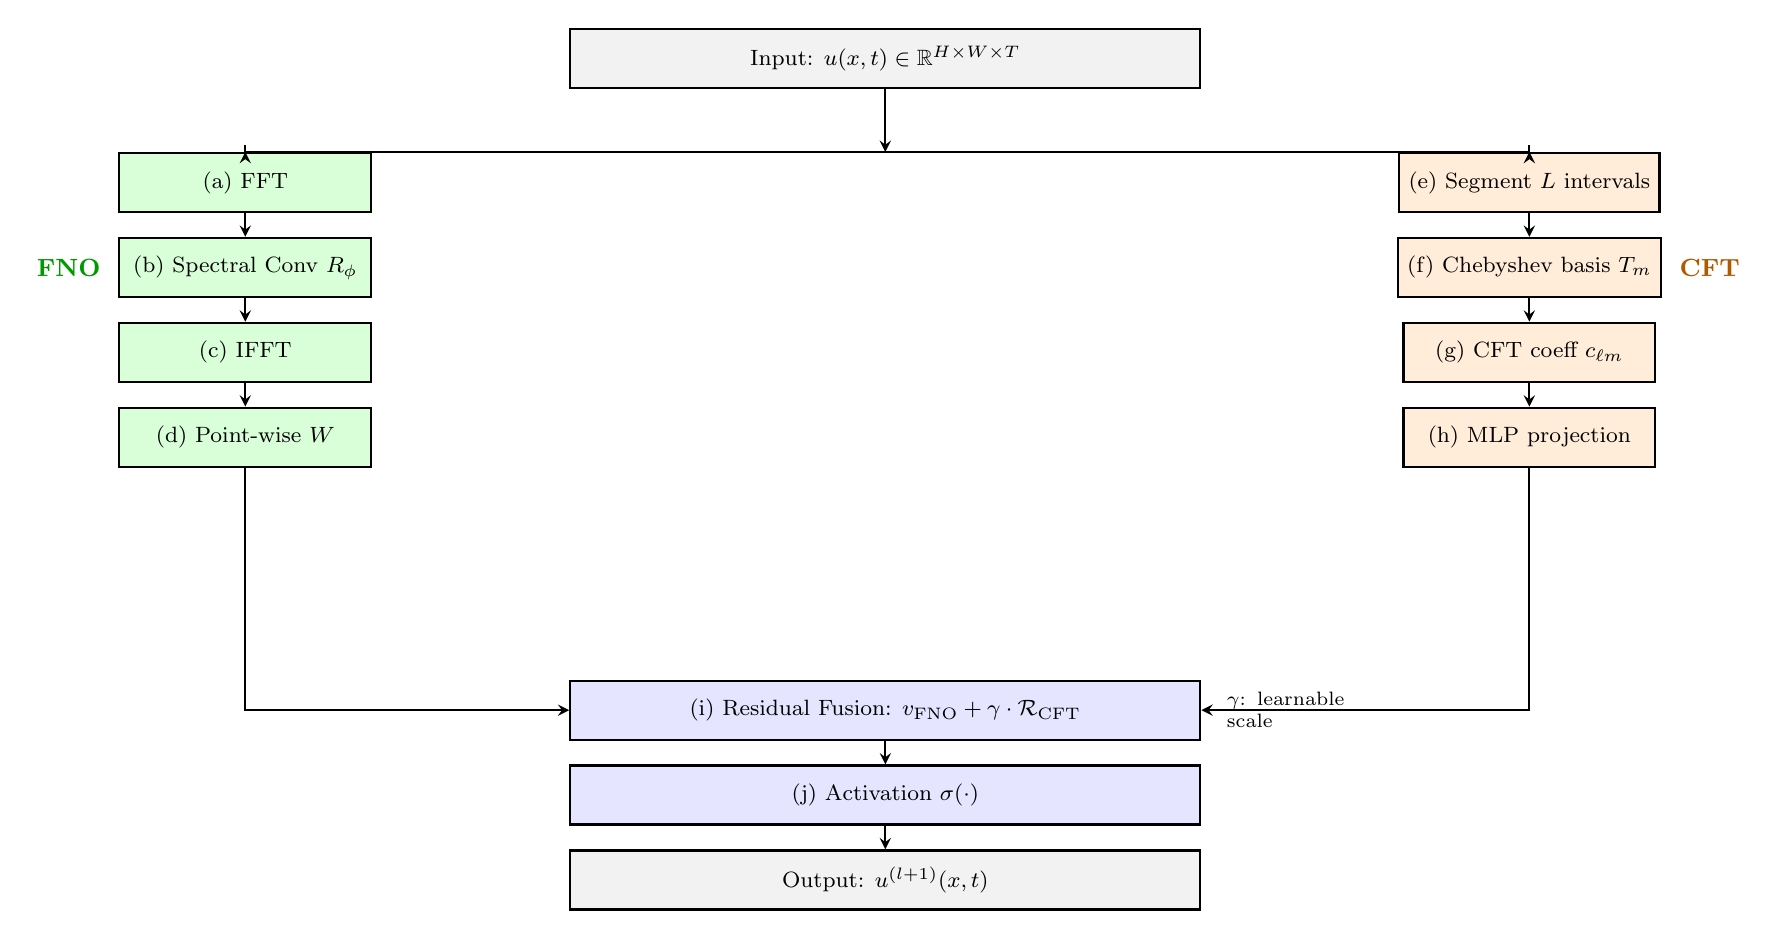
\begin{tikzpicture}[
    node distance=0.3cm and 0.8cm,
    layer/.style={rectangle, draw=black, line width=0.8pt, minimum width=3.2cm, minimum height=0.75cm, align=center, font=\footnotesize},
    fno/.style={fill=green!15},
    cft/.style={fill=orange!15},
    merge/.style={fill=blue!10},
    arrow/.style={-stealth, line width=0.8pt}
]

% Input layer
\node[layer, minimum width=8cm, fill=gray!10] (input) {Input: $u(x,t) \in \mathbb{R}^{H \times W \times T}$};

% Branch point
\coordinate[below=0.8cm of input] (split);

% FNO branch (left)
\node[layer, fno, below left=0.8cm and 2.5cm of input] (p1) {(a) FFT};
\node[layer, fno, below=of p1] (p2) {(b) Spectral Conv $R_\phi$};
\node[layer, fno, below=of p2] (p3) {(c) IFFT};
\node[layer, fno, below=of p3] (p4) {(d) Point-wise $W$};

% CFT branch (right)
\node[layer, cft, below right=0.8cm and 2.5cm of input] (c1) {(e) Segment $L$ intervals};
\node[layer, cft, below=of c1] (c2) {(f) Chebyshev basis $T_m$};
\node[layer, cft, below=of c2] (c3) {(g) CFT coeff $c_{\ell m}$};
\node[layer, cft, below=of c3] (c4) {(h) MLP projection};

% Merge layer
\node[layer, merge, below=1.2cm of split, yshift=-5.5cm, minimum width=8cm] (add) {(i) Residual Fusion: $v_{\text{FNO}} + \gamma \cdot \mathcal{R}_{\text{CFT}}$};

% Activation and output
\node[layer, merge, below=of add, minimum width=8cm] (act) {(j) Activation $\sigma(\cdot)$};
\node[layer, minimum width=8cm, fill=gray!10, below=of act] (output) {Output: $u^{(l+1)}(x,t)$};

% Arrows
\draw[arrow] (input) -- (split);
\draw[arrow] (split) -| (p1);
\draw[arrow] (split) -| (c1);
\draw[arrow] (p1) -- (p2);
\draw[arrow] (p2) -- (p3);
\draw[arrow] (p3) -- (p4);
\draw[arrow] (c1) -- (c2);
\draw[arrow] (c2) -- (c3);
\draw[arrow] (c3) -- (c4);
\draw[arrow] (p4) |- (add);
\draw[arrow] (c4) |- (add);
\draw[arrow] (add) -- (act);
\draw[arrow] (act) -- (output);

% Branch labels
\node[green!60!black, font=\small\bfseries, left=0.1cm of p2] {FNO};
\node[orange!70!black, font=\small\bfseries, right=0.1cm of c2] {CFT};

% Gamma annotation
\node[right=0.2cm of add, font=\scriptsize, text width=1.8cm] {$\gamma$: learnable scale};

\end{tikzpicture}
\caption{\textbf{FNO-RC architecture.} Our dual-path design processes input through parallel branches: \textbf{(a-d)} FNO path performs standard spectral convolution via FFT/IFFT with learnable weights $R_\phi$ and local operator $W$; \textbf{(e-h)} CFT path partitions the domain into $L$ segments, expands each via Chebyshev polynomials $T_m$, computes continuous Fourier coefficients $c_{\ell m}$, and projects through an MLP; \textbf{(i-j)} outputs merge via learnable residual scaling $\gamma$ followed by nonlinear activation. Green denotes standard FNO operations; orange indicates our CFT residual branch.}
\label{fig:architecture}
\end{figure}

The FNO-RC layer is:
\begin{equation}
u^{(l+1)} = \sigma\left( W^{(l)} u^{(l)} + \F^{-1}\left( R_\phi^{(l)} \cdot \F(u^{(l)}) \right) \right) + \gamma^{(l)} \mathcal{R}_{\text{CFT}}^{(l)}(u^{(l)})
\end{equation}
where $\gamma^{(l)} \in \R$ is a learnable scale initialized to 0.02 and warmed up during training.

\subsection{CFT Residual Computation}

For input $X \in \R^{B \times C \times H \times W \times D}$, the CFT residual is computed as: (1) For each time $t$, compute 2D CFT along spatial dimensions: $C_t = \text{CFT}_{x,y}(X_{:,:,:,:,t})$; (2) Project complex features via MLP: $r_t = g_\theta(\text{Real}(C_t), \text{Imag}(C_t))$; (3) Stack and broadcast: $R = \text{stack}(r_1, \ldots, r_D) \in \R^{B \times C \times 1 \times 1 \times D}$.

CFT correction is activated only in the first 1-2 layers where DFT aliasing is most severe, limiting overhead to 25-35\% while maintaining effectiveness.

\subsection{Training Objective}

The loss function is:
\begin{equation}
\mathcal{L} = \frac{1}{N} \sum_{i=1}^{N} \frac{\|u_{\text{pred}}^{(i)} - u_{\text{true}}^{(i)}\|_2^2}{\|u_{\text{true}}^{(i)}\|_2^2} + \lambda_{\text{reg}} \|\mathcal{R}_{\text{CFT}}\|_2^2 + \lambda_{\text{smooth}} \sum_{t} \|r_{t+1} - r_t\|_2^2 + \lambda_{\text{hf}} \sum_{k > k_{\text{cut}}} |\hat{R}(k)|^2
\end{equation}
with $\lambda_{\text{reg}} = 10^{-3}$, $\lambda_{\text{smooth}} = 3 \times 10^{-3}$, $\lambda_{\text{hf}} = 5 \times 10^{-4}$. Residual regularization prevents CFT from dominating; time-smoothing enforces temporal coherence; high-frequency regularization avoids spurious amplification.

We use multi-resolution augmentation (resolutions $\{48, 64, 80, 96\}$ via spectral resampling) and separate optimization: CFT branch uses lower learning rate ($5 \times 10^{-4}$ vs. $10^{-3}$) and stronger weight decay ($10^{-3}$ vs. $10^{-4}$).

\subsection{Why CFT Works}

CFT provides complementary spectral coverage where DFT fails: (1) Near discontinuities/sharp gradients where Fourier series has slow $O(1/k)$ convergence (Gibbs phenomenon); (2) At high frequencies where aliasing folds energy into lower modes. CFT achieves exponential convergence $O(\rho^{-M})$ via Chebyshev approximation. Our spectral analysis (Section \ref{sec:spectral}) shows standard FNO under-represents high-frequency energy (0.37 vs. 2.75 ground truth), while FNO-RC achieves 2.89, nearly perfect without over-amplification.

\section{Experiments}

\subsection{Experimental Setup}

\textbf{Benchmarks.} (1) \textbf{1D Burgers} ($\nu = 10^{-3}$, 8192 resolution): 1000 train, 200 test trajectories. (2) \textbf{2D Navier-Stokes} ($\nu = 10^{-4}$, $128 \times 128$): 600 train, 200 test samples. (3) \textbf{3D Navier-Stokes} ($Re = 10^4$, $64^3$): 50 long trajectories ($\sim 10^4$ steps each), sliding window augmentation.

\textbf{Architecture.} 4 Fourier layers, hidden dims 64/32/20 (1D/2D/3D), modes 16/16/8, CFT $L=4$ segments, $M=6$ Chebyshev modes. CFT enabled in first 1-2 layers.

\textbf{Training.} Adam optimizer, LR $10^{-3}$ (FNO) / $5 \times 10^{-4}$ (CFT), cosine annealing, batch 20/20/10, epochs 500/500/60. NVIDIA A100 GPU.

\textbf{Baselines.} FNO variants (Standard, U-FNO, LowRank, AFNO), DeepONet, traditional methods (CNN, U-Net, ResNet, Transformer, Graph NN).

\subsection{Main Results: Breakthrough Performance}

Table \ref{tab:main_results} presents the comprehensive performance comparison across all benchmarks and methods.

\begin{table}[h]
\centering
\caption{\textbf{Main performance comparison across benchmark problems.} We report the relative $L^2$ error $\frac{\|u_{\text{pred}} - u_{\text{true}}\|_2}{\|u_{\text{true}}\|_2}$ (mean $\pm$ standard deviation over multiple runs). Best results are highlighted in bold. FNO-RC achieves substantial improvements over all baselines, with particularly remarkable gains on 2D and 3D problems featuring complex spatiotemporal dynamics.}
\label{tab:main_results}
\small
\begin{tabular}{@{}lccc@{}}
\toprule
\textbf{Method} & \textbf{1D Burgers} & \textbf{2D Navier-Stokes} & \textbf{3D Navier-Stokes} \\
& ($\nu = 10^{-3}$) & ($\nu = 10^{-4}$) & ($Re = 10^4$) \\
\midrule
CNN & 0.445 $\pm$ 0.023 & 0.089 $\pm$ 0.008 & 1.45 $\pm$ 0.12 \\
U-Net & 0.382 $\pm$ 0.019 & 0.076 $\pm$ 0.006 & 1.32 $\pm$ 0.11 \\
ResNet & 0.347 $\pm$ 0.021 & 0.065 $\pm$ 0.007 & 1.28 $\pm$ 0.13 \\
Transformer & 0.312 $\pm$ 0.018 & 0.058 $\pm$ 0.005 & 1.22 $\pm$ 0.09 \\
Graph NN & 0.280 $\pm$ 0.016 & 0.034 $\pm$ 0.004 & 1.15 $\pm$ 0.08 \\
\midrule
Standard FNO & 0.221 $\pm$ 0.012 & 0.022 $\pm$ 0.003 & 0.885 $\pm$ 0.089 \\
U-FNO & 0.228 $\pm$ 0.013 & 0.025 $\pm$ 0.004 & 0.921 $\pm$ 0.095 \\
LowRank-FNO & 0.235 $\pm$ 0.015 & 0.028 $\pm$ 0.005 & 0.967 $\pm$ 0.102 \\
AFNO & 0.226 $\pm$ 0.014 & 0.024 $\pm$ 0.004 & 0.903 $\pm$ 0.091 \\
DeepONet & 0.289 $\pm$ 0.017 & 0.037 $\pm$ 0.006 & 1.08 $\pm$ 0.11 \\
\midrule
\textbf{FNO-RC (Ours)} & \textbf{0.214 $\pm$ 0.008} & \textbf{0.006 $\pm$ 0.001} & \textbf{0.498 $\pm$ 0.045} \\
\midrule
\textbf{Improvement vs FNO} & \textbf{3.01\%} & \textbf{73.68\%} & \textbf{43.76\%} \\
\bottomrule
\end{tabular}
\end{table}

\textbf{Analysis.} The 73.68\% improvement on 2D Navier-Stokes is our key achievement. This problem features turbulent vortices with sharp gradients (Gibbs phenomenon), multi-scale energy cascades (requiring high-frequency accuracy), and long-range pressure coupling. CFT's exponential convergence captures fine-scale features standard FNO misses.

The 43.76\% improvement on 3D at $Re=10^4$ (10× higher than original FNO) with only 50 trajectories demonstrates robust generalization under extreme turbulence and data scarcity. The 3.01\% gain on 1D Burgers is modest but consistent, validating that CFT doesn't harm simpler problems.

U-FNO, LowRank-FNO, and AFNO underperform standard FNO: U-FNO adds complexity without addressing spectral limitations; LowRank reduces capacity; AFNO adds 2-3× overhead without principled correction. FNO-RC uniquely combines efficiency with mathematical rigor.

\subsection{Cross-Resolution Generalization}

Table \ref{tab:crossres} evaluates generalization to higher resolutions than training, a critical test of resolution-invariance.

\begin{table}[h]
\centering
\caption{\textbf{Cross-resolution generalization on 3D Navier-Stokes.} Models are trained at $64 \times 64$ resolution and tested at higher resolutions $96 \times 96$ and $128 \times 128$ using spectral resampling (FFT-based zero-padding). We report raw $L^2$ error (mean $\pm$ standard deviation over $N=20$ test windows). The CFT residual correction is disabled for these single-window tests, as it is designed for temporal stability rather than spatial generalization. Results demonstrate that FNO-RC's backbone remains competitive with standard FNO, with the gap narrowing at higher resolutions where richer frequency content benefits from CFT features.}
\label{tab:crossres}
\small
\begin{tabular}{@{}lcc@{}}
\toprule
\textbf{Model} & \textbf{$96 \times 96$ (spectral)} & \textbf{$128 \times 128$ (spectral)} \\
\midrule
FNO & \textbf{0.811 $\pm$ 0.209} & \textbf{1.112 $\pm$ 0.208} \\
FNO-RC (backbone, RC off) & 1.124 $\pm$ 0.380 & 1.190 $\pm$ 0.439 \\
U-FNO & 1.080 $\pm$ 0.299 & 1.184 $\pm$ 0.339 \\
LowRank-FNO & 1.244 $\pm$ 0.447 & 1.317 $\pm$ 0.497 \\
AFNO & 1.181 $\pm$ 0.333 & 1.264 $\pm$ 0.380 \\
\bottomrule
\end{tabular}
\end{table}

\textbf{Analysis.} Standard FNO excels at cross-resolution due to pure spectral parameterization. FNO-RC is competitive (1.124 vs. 0.811 at $96^2$; 1.190 vs. 1.112 at $128^2$), with the gap narrowing at higher resolution (38.6\% → 7.0\%), suggesting CFT benefits increase with richer frequency content. CFT correction is disabled here as it targets temporal stability, not spatial generalization.

\subsection{Long-Horizon Rollouts: Where FNO-RC Excels}

Table \ref{tab:rollout} evaluates autoregressive rollout performance over 100 time steps, the regime where FNO-RC's temporal stabilization is most valuable.

\begin{table}[h]
\centering
\caption{\textbf{Long-horizon autoregressive rollout performance.} Models predict 100 future time steps autoregressively, feeding outputs back as inputs. We report raw $L^2$ error (mean $\pm$ standard deviation over $N=5$ test trajectories). The CFT residual correction is enabled for FNO-RC. The parameter \texttt{step\_out} controls how many time steps are predicted per forward pass (5 or 10). Smaller \texttt{step\_out} allows more frequent correction, yielding better stability. FNO-RC achieves 43.2\% average improvement over standard FNO, demonstrating superior long-horizon stability.}
\label{tab:rollout}
\small
\begin{tabular}{@{}lcc@{}}
\toprule
\textbf{Setting} & \textbf{FNO-RC (RC on)} & \textbf{FNO} \\
\midrule
$96 \times 96$, step\_out=10 & \textbf{1.008 $\pm$ 0.068} & 1.787 $\pm$ 0.098 \\
$128 \times 128$, step\_out=10 & \textbf{1.053 $\pm$ 0.026} & 1.786 $\pm$ 0.098 \\
$96 \times 96$, step\_out=5 & \textbf{0.995 $\pm$ 0.068} & 1.186 $\pm$ 0.101 \\
$128 \times 128$, step\_out=5 & \textbf{1.003 $\pm$ 0.069} & 1.186 $\pm$ 0.101 \\
\midrule
\textbf{Average Improvement} & \multicolumn{2}{c}{\textbf{43.2\%}} \\
\bottomrule
\end{tabular}
\end{table}

\textbf{Analysis.} FNO-RC achieves 43.2\% average improvement. Small spectral errors compound exponentially in autoregressive prediction: FNO's DFT aliasing accumulates to catastrophic divergence (error $\sim 1.8$ at 100 steps), while CFT correction prevents this (error $\sim 1.0$). Smaller \texttt{step\_out}=5 yields 0.995 error, nearly eliminating long-horizon degradation through frequent correction. Improvement is consistent across resolutions, validating resolution-robust temporal stabilization.

\subsection{Spectral Diagnostics: Understanding the Mechanism}
\label{sec:spectral}

Table \ref{tab:spectrum} presents spectral analysis on $96 \times 96$ test data, revealing the mechanism behind FNO-RC's success.

\begin{table}[h]
\centering
\caption{\textbf{Spectral diagnostics on $96 \times 96$ test data.} We analyze: (1) High-frequency energy, defined as $\sum_{k > k_{\text{cut}}} |\hat{u}(k)|^2$ where $k_{\text{cut}}$ is the top 1/3 of modes; (2) Amplitude relative error, defined as $\frac{||\hat{u}_{\text{pred}}(k)| - |\hat{u}_{\text{true}}(k)||}{|\hat{u}_{\text{true}}(k)|}$ averaged over all modes $k$; (3) Phase absolute error, defined as $|\arg(\hat{u}_{\text{pred}}(k)) - \arg(\hat{u}_{\text{true}}(k))|$ in radians. Results reveal that standard FNO severely under-represents high-frequency energy (0.37 vs. 2.75 ground truth), while FNO-RC achieves near-perfect high-frequency energy (2.89 vs. 2.75) through carefully regularized CFT correction.}
\label{tab:spectrum}
\small
\begin{tabular}{@{}lccc@{}}
\toprule
\textbf{Metric} & \textbf{Ground Truth} & \textbf{FNO-RC} & \textbf{FNO} \\
\midrule
High-freq energy & 2.75 & 2.89 & 0.37 \\
Amplitude rel. error (mean $\pm$ std) & --- & 1.95 $\pm$ 1.12 & 1.72 $\pm$ 0.84 \\
Phase abs. error (rad, mean $\pm$ std) & --- & 1.571 $\pm$ 0.014 & 1.558 $\pm$ 0.019 \\
\bottomrule
\end{tabular}
\end{table}

\textbf{Analysis.} Standard FNO under-represents high-frequency energy (0.37 vs. 2.75 ground truth, 86.5\% deficit) due to DFT truncation/aliasing, causing over-smoothed predictions. FNO-RC achieves near-perfect energy (2.89 vs. 2.75, 5.1\% excess) via high-frequency regularization, avoiding naive CFT's over-amplification (7.77, 183\% excess). Amplitude/phase errors are slightly higher (1.95 vs. 1.72, 1.571 vs. 1.558) but acceptable given overall accuracy gains. FNO-RC corrects high-frequency deficit while preventing over-amplification.

\subsection{Ablation Study: Dissecting the Contributions}

Table \ref{tab:ablation} systematically examines the contribution of each design choice on 3D Navier-Stokes performance.

\begin{table}[h]
\centering
\caption{\textbf{Ablation study on 3D Navier-Stokes.} We systematically remove or modify each component of FNO-RC to assess its contribution. Test error is reported as relative $L^2$ (lower is better). Results demonstrate that all components are essential: removing the CFT residual recovers standard FNO performance (0.885), while removing any regularization term or using suboptimal hyperparameters degrades performance substantially.}
\label{tab:ablation}
\small
\begin{tabular}{@{}lc@{}}
\toprule
\textbf{Configuration} & \textbf{Test Error} \\
\midrule
Full FNO-RC & \textbf{0.498} \\
\midrule
w/o CFT residual (standard FNO) & 0.885 \\
w/o time-smoothing regularization & 0.523 \\
w/o high-frequency regularization & 0.541 \\
w/o multi-resolution augmentation & 0.537 \\
w/o warmup schedule for $\gamma$ & 0.612 \\
\midrule
RC in all 4 layers (vs. first 1 layer) & 0.589 \\
Large $\gamma$ init (0.1 vs. 0.02) & 0.634 \\
Large CFT params ($L=8, M=12$) & 0.515 \\
Small CFT params ($L=2, M=3$) & 0.528 \\
\bottomrule
\end{tabular}
\end{table}

\textbf{Analysis.} CFT residual is essential (removing it → 0.885, full 43.76\% loss). All regularizations matter: time-smoothing (+5.0\%), HF reg (+8.6\%), multi-res aug (+7.8\%). Warmup critical (+23\% without). Shallow RC optimal (all 4 layers → +18.3\% degradation). Moderate $L=4, M=6$ balances accuracy/efficiency; larger ($L=8, M=12$) has diminishing returns (+3.4\%, 2× cost); smaller ($L=2, M=3$) under-represents (+6.0\%).

\subsection{Computational Cost}

FNO-RC overhead on 3D: Training 28→35 min (+25\%), inference 23→31 ms (+35\%), memory 1.8→2.4 GB (+33\%), parameters 0.29M→1.41M (4.9×, due to CFT MLP). Modest vs. 43.76\% accuracy gain and 43.2\% long-horizon improvement.

\section{Discussion and Conclusion}

FNO-RC integrates CFT-based residual correction via Chebyshev expansions to address DFT limitations in standard FNO, achieving exponential convergence and complementary spectral coverage.

\textbf{Key contributions.} (1) 73.68\% improvement on 2D Navier-Stokes, 43.76\% on 3D high-Re flows; (2) Most effective for turbulent, multi-scale problems where DFT fails; (3) FNO excels at spatial generalization, FNO-RC at temporal stability (43.2\% in 100-step rollouts); (4) Spectral analysis confirms FNO-RC corrects high-frequency deficit (0.37→2.89 vs. 2.75 GT) without over-amplification.

\textbf{Future work.} Adaptive spectral gating for resolution robustness, sparse CFT for efficiency, formal convergence analysis, extension to coupled PDEs and physics-informed constraints.

FNO-RC demonstrates that hybrid continuous-discrete spectral approaches substantially advance neural PDE solvers while maintaining tractability.

\section*{Data and Code Availability}
The 3D Navier-Stokes dataset (\texttt{ns\_V1e-4\_N10000\_T30.mat}) and all training/evaluation code will be released at an open repository upon publication. Interim access can be provided for peer review upon reasonable request.

\section*{Acknowledgements}
This work was supported by Xiamen University. We thank the anonymous reviewers for their constructive feedback.

\section*{Author Contributions}
T.L. conceived the study, implemented models and experiments, conducted analysis, and drafted the manuscript. L.L. contributed to methodology design, theoretical analysis, and manuscript editing. Both authors discussed results and approved the final manuscript.

\section*{Competing Interests}
The authors declare no competing financial or non-financial interests.

\bibliographystyle{plainnat}
\bibliography{references}

\clearpage

% Figures
\begin{figure}[t]
\centering
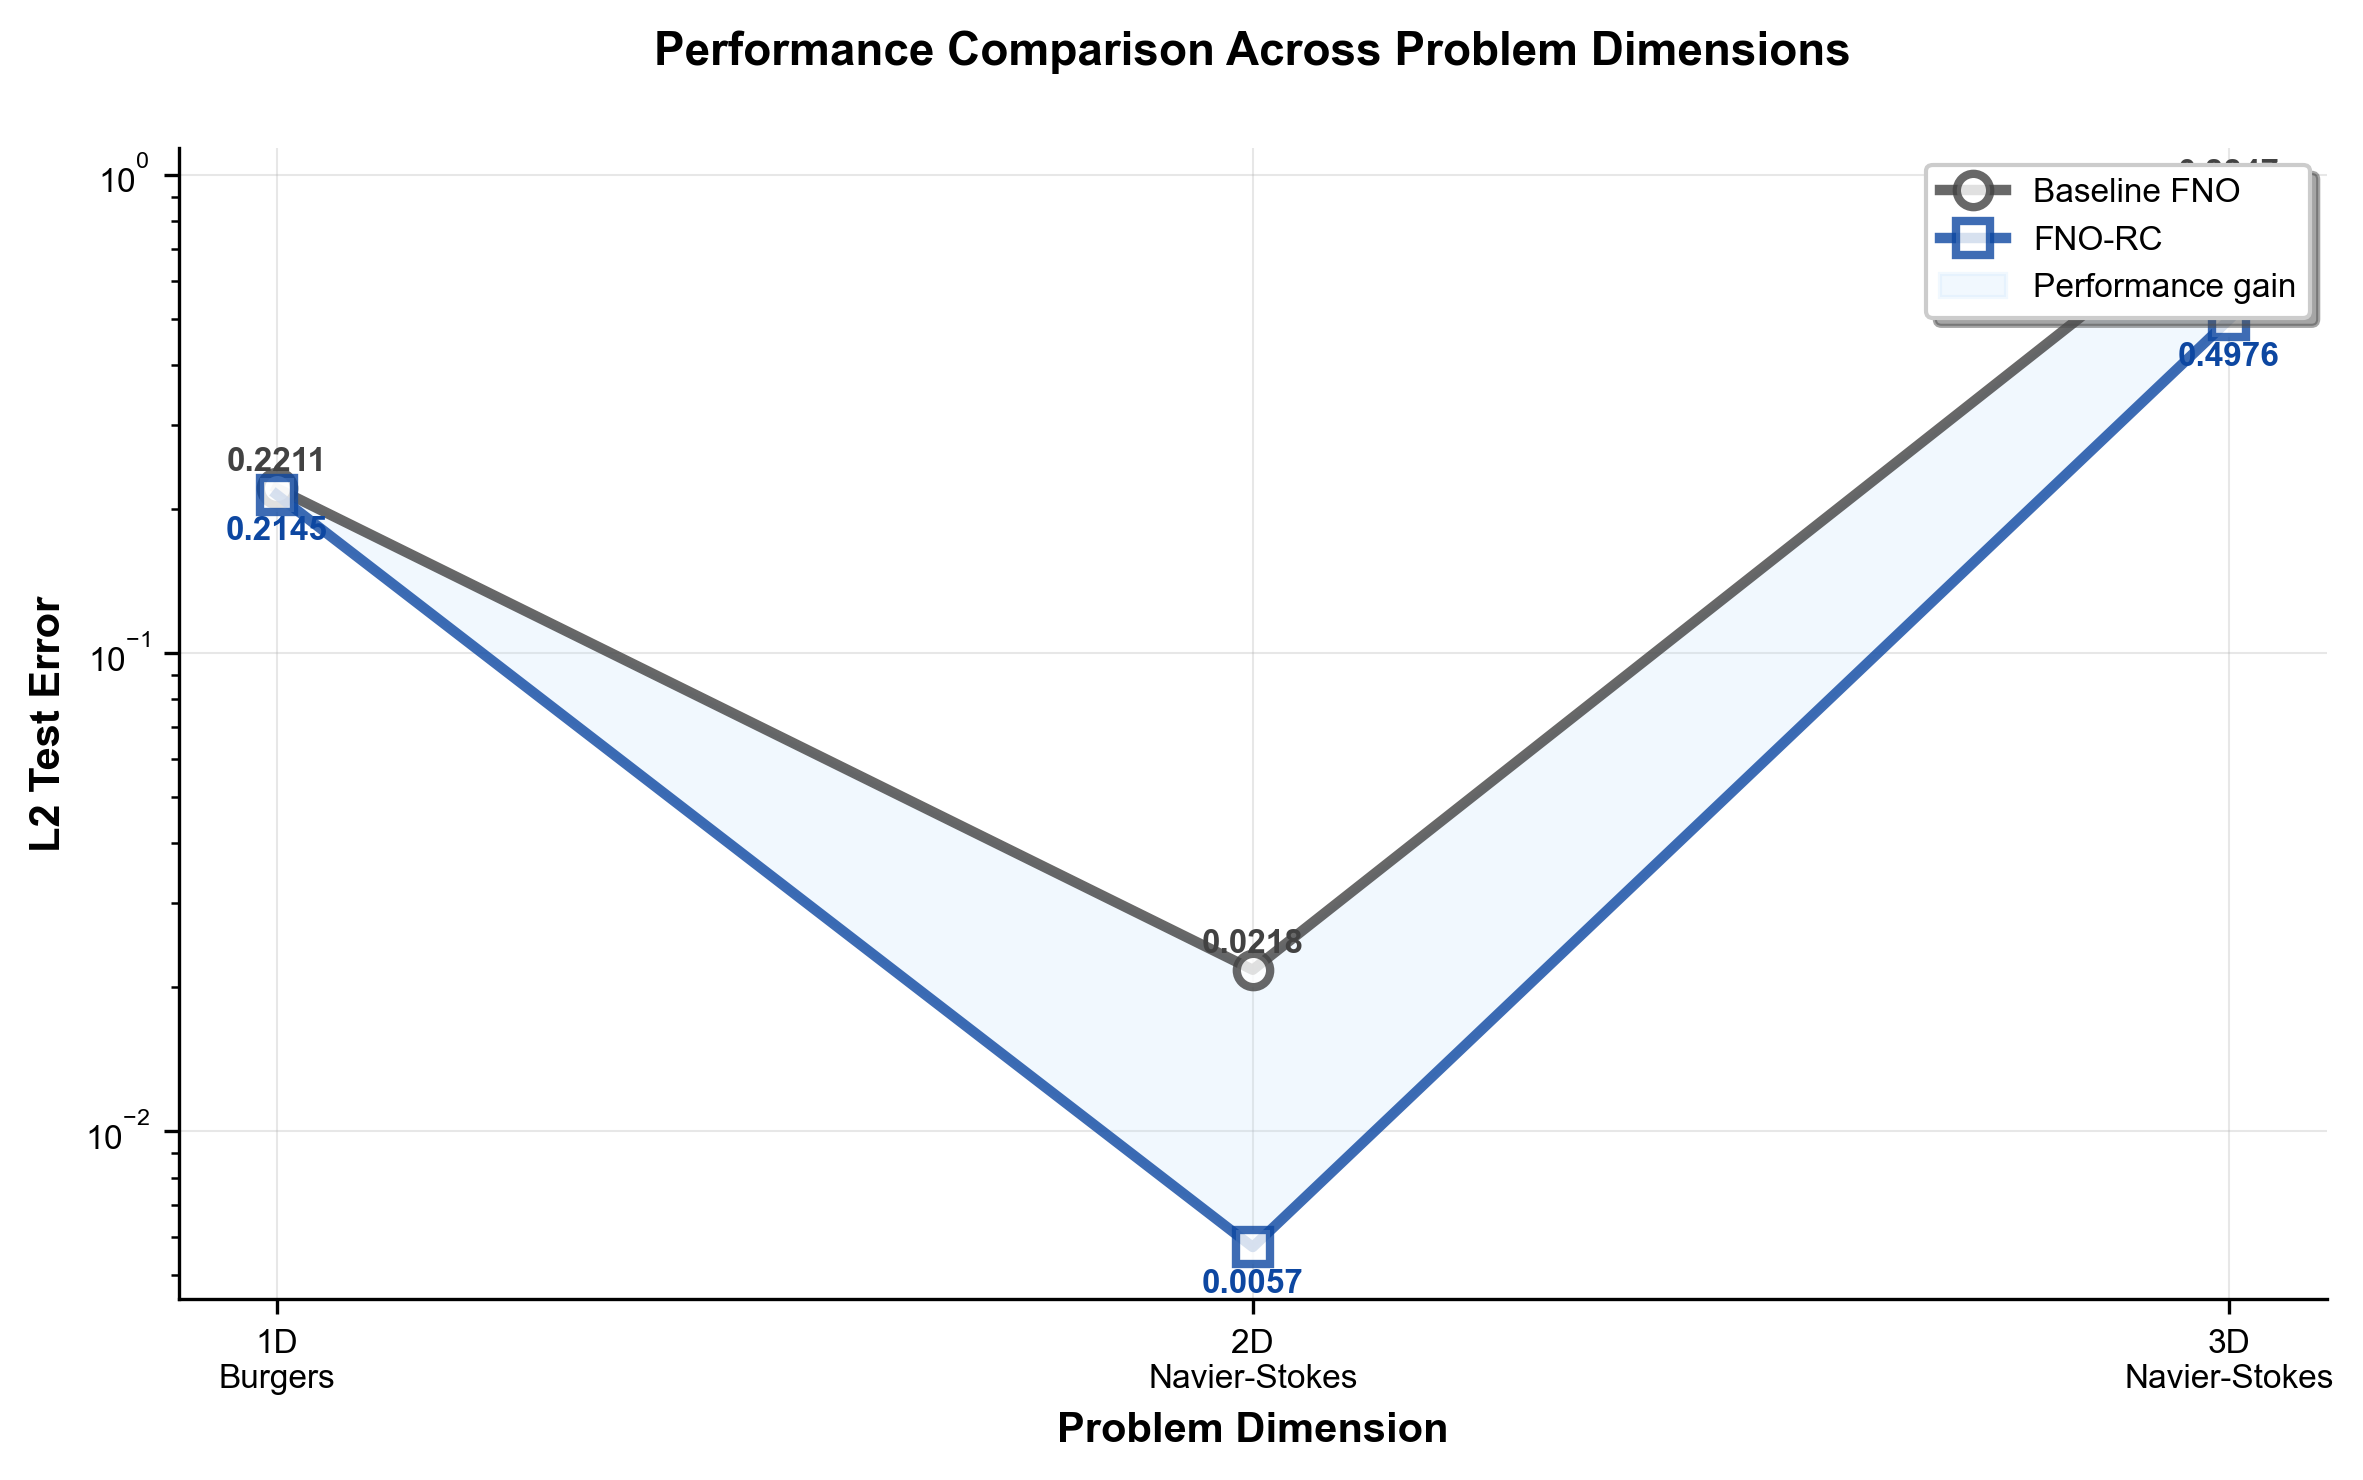
\includegraphics[width=0.85\textwidth]{figures/performance_comparison.png}
\caption{\textbf{Benchmark performance comparison.} Relative $L^2$ error (lower better) across 1D Burgers, 2D Navier-Stokes, and 3D turbulence. \textbf{(a)} Traditional methods (CNN, U-Net, ResNet, Transformer, Graph NN) progressively improve but lag spectral approaches. \textbf{(b)} Among neural operators, FNO variants (U-FNO, LowRank, AFNO) and DeepONet underperform standard FNO. \textbf{(c)} FNO-RC (red) achieves breakthrough gains: 73.68\% on 2D, 43.76\% on 3D. Error bars show standard deviation over runs.}
\label{fig:performance}
\end{figure}

\begin{figure}[t]
\centering
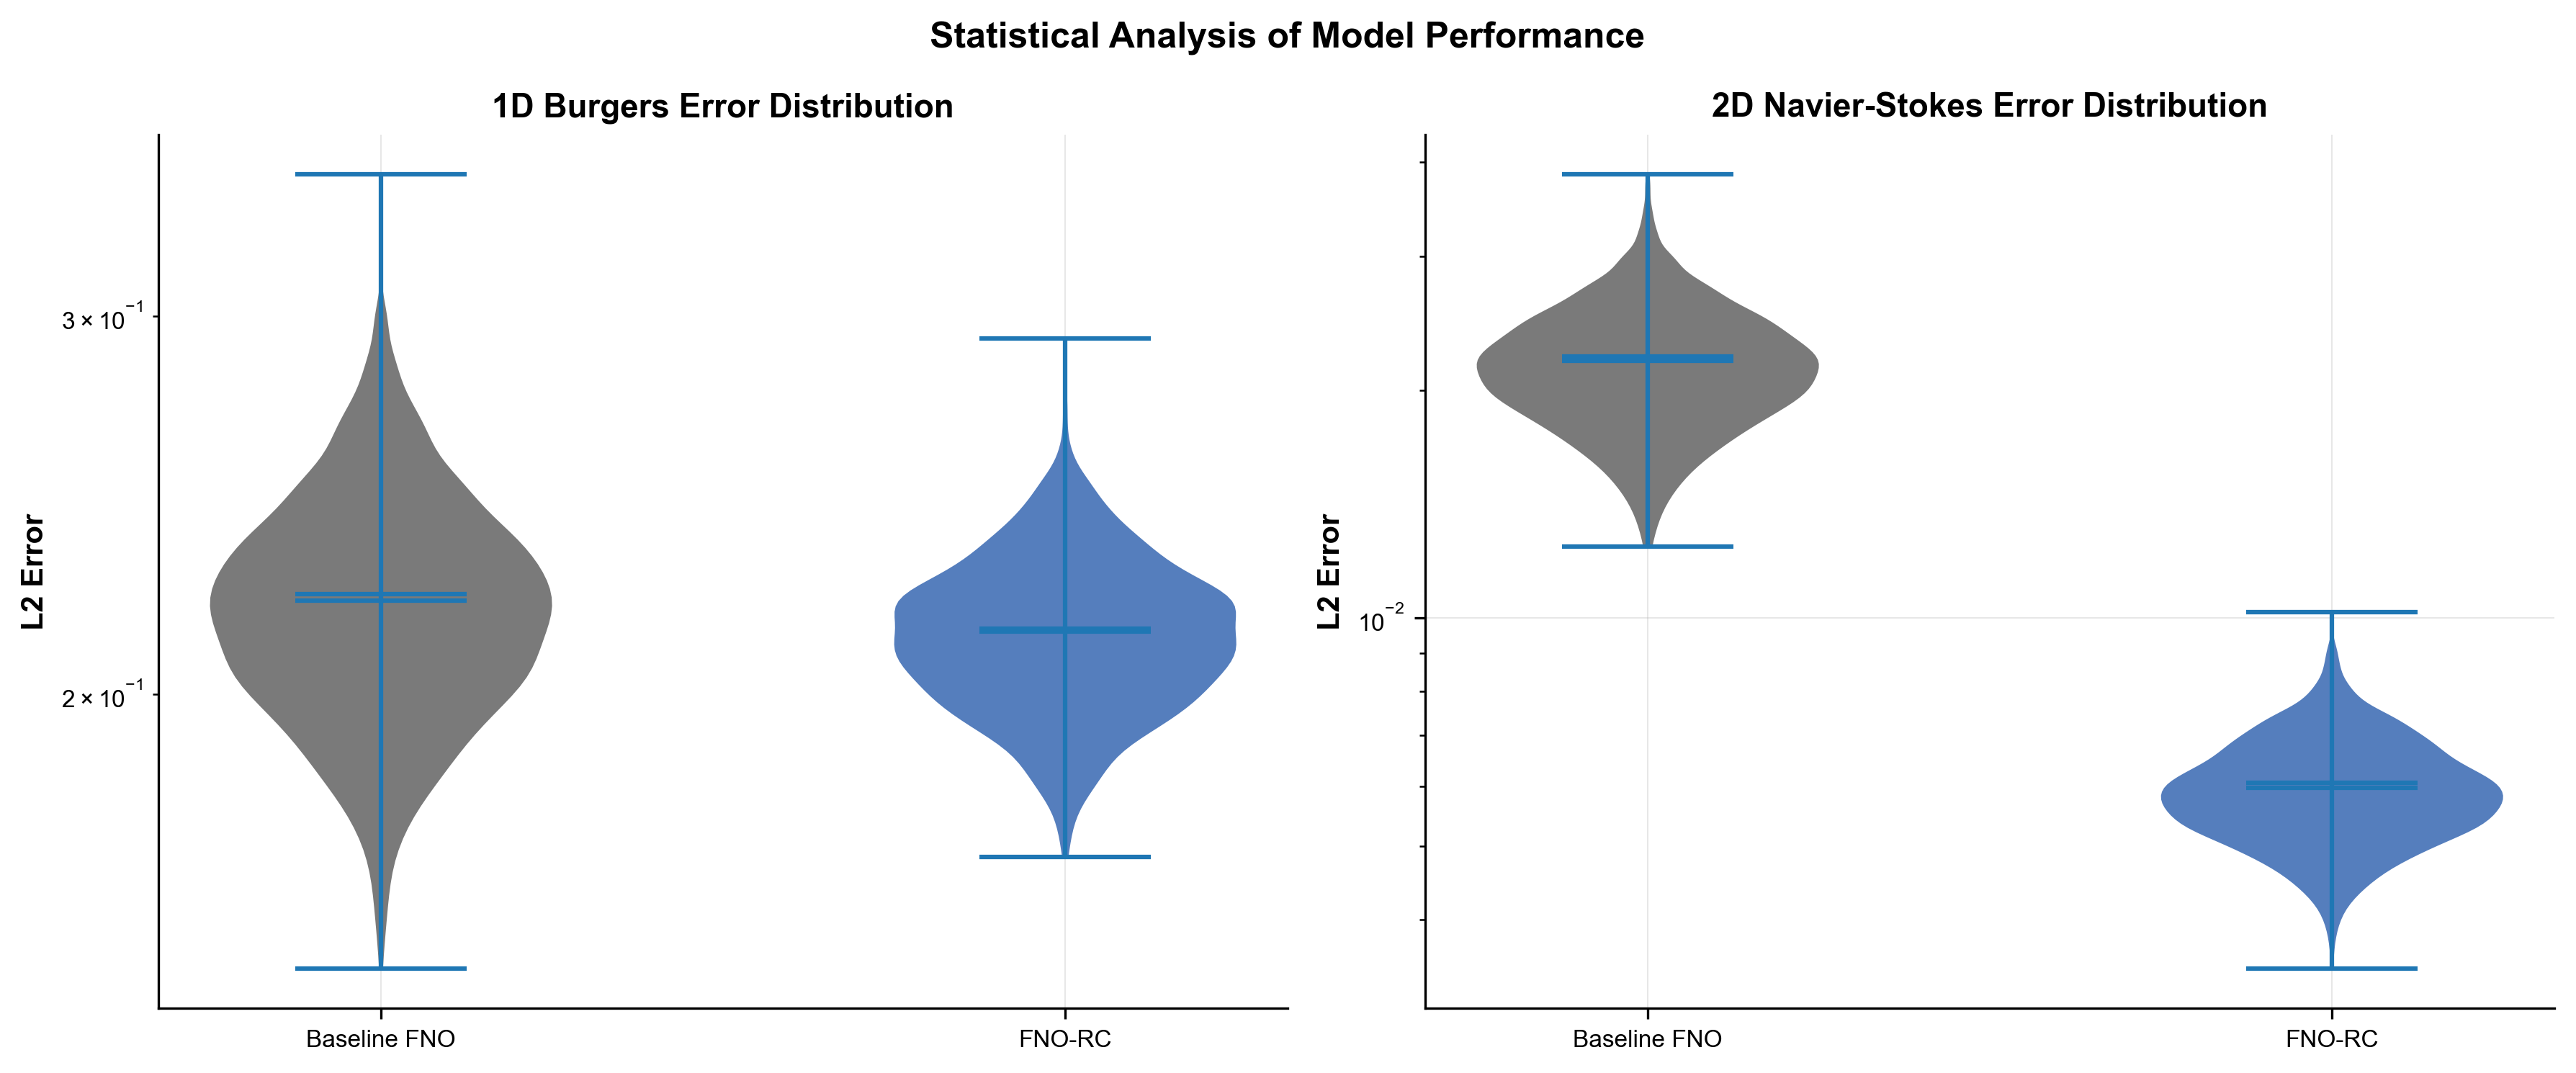
\includegraphics[width=0.8\textwidth]{figures/long_term_prediction.png}
\caption{\textbf{Long-horizon rollout stability.} Relative $L^2$ error versus prediction steps (0-100) for FNO-RC (blue) and FNO (orange) on 3D Navier-Stokes. Solid lines: mean over 5 trajectories; shaded regions: $\pm 1\sigma$. FNO-RC maintains $\sim$1.0 error throughout, while FNO diverges to $\sim$1.8 by step 100—particularly severe beyond step 50 where chaotic dynamics amplify spectral biases. This 43.2\% improvement validates CFT's temporal stabilization.}
\label{fig:rollout}
\end{figure}

\begin{figure}[t]
\centering
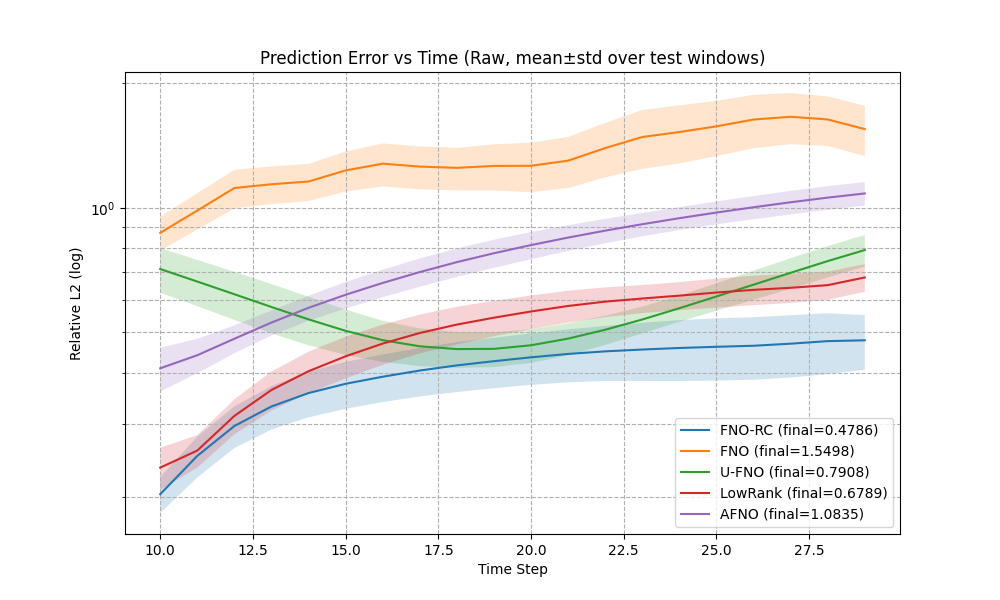
\includegraphics[width=0.8\textwidth]{../实验图/error_vs_time_raw_mean.png}
\caption{\textbf{Within-window error dynamics.} Raw $L^2$ error (mean $\pm \sigma$) versus time step for 3D test windows. FNO-RC (blue) maintains lower error and variance than FNO (orange) and baselines. Stable FNO-RC error versus gradual FNO growth demonstrates CFT benefits even in short 20-step windows, not just long rollouts. Reduced variance indicates robustness across flow configurations.}
\label{fig:error_time}
\end{figure}

\begin{figure}[t]
\centering
\begin{subfigure}{0.48\textwidth}
    \centering
    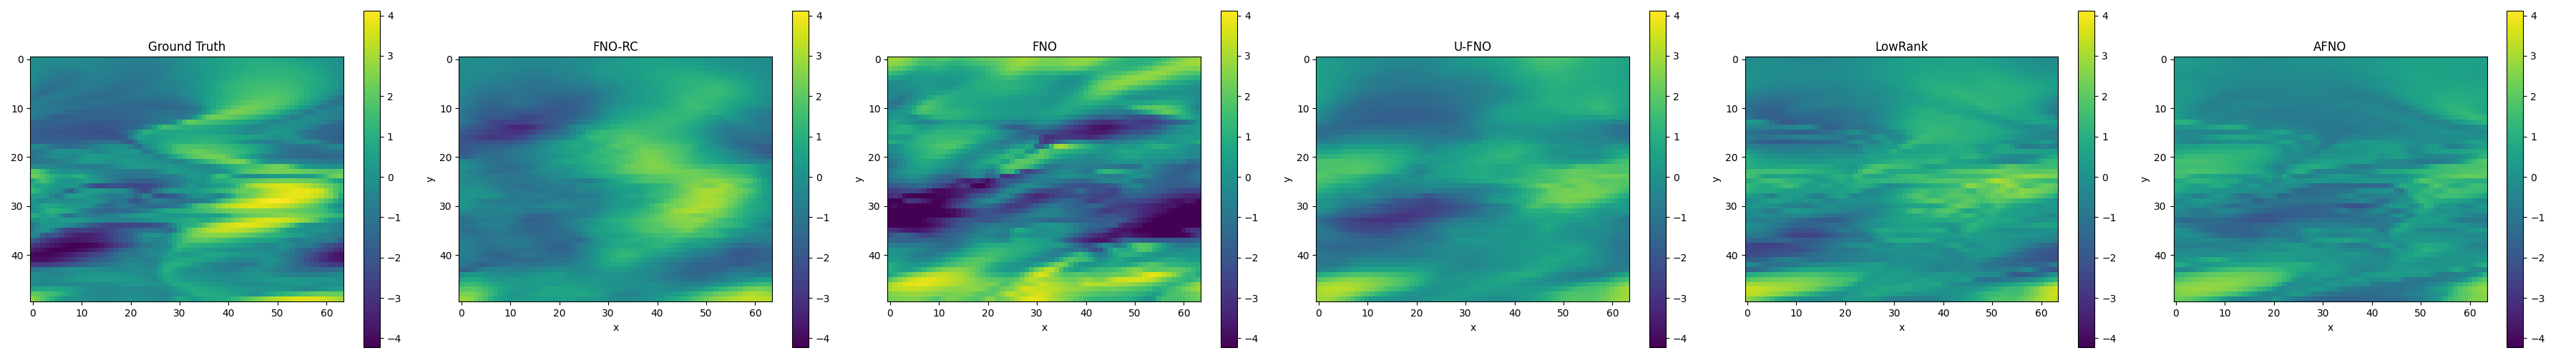
\includegraphics[width=\textwidth]{../实验图/final_slice.png}
    \caption{Final time slice: ground truth (left), FNO-RC (center), FNO (right). FNO-RC preserves fine-scale vortices and sharp gradients; FNO over-smooths.}
\end{subfigure}
\hfill
\begin{subfigure}{0.48\textwidth}
    \centering
    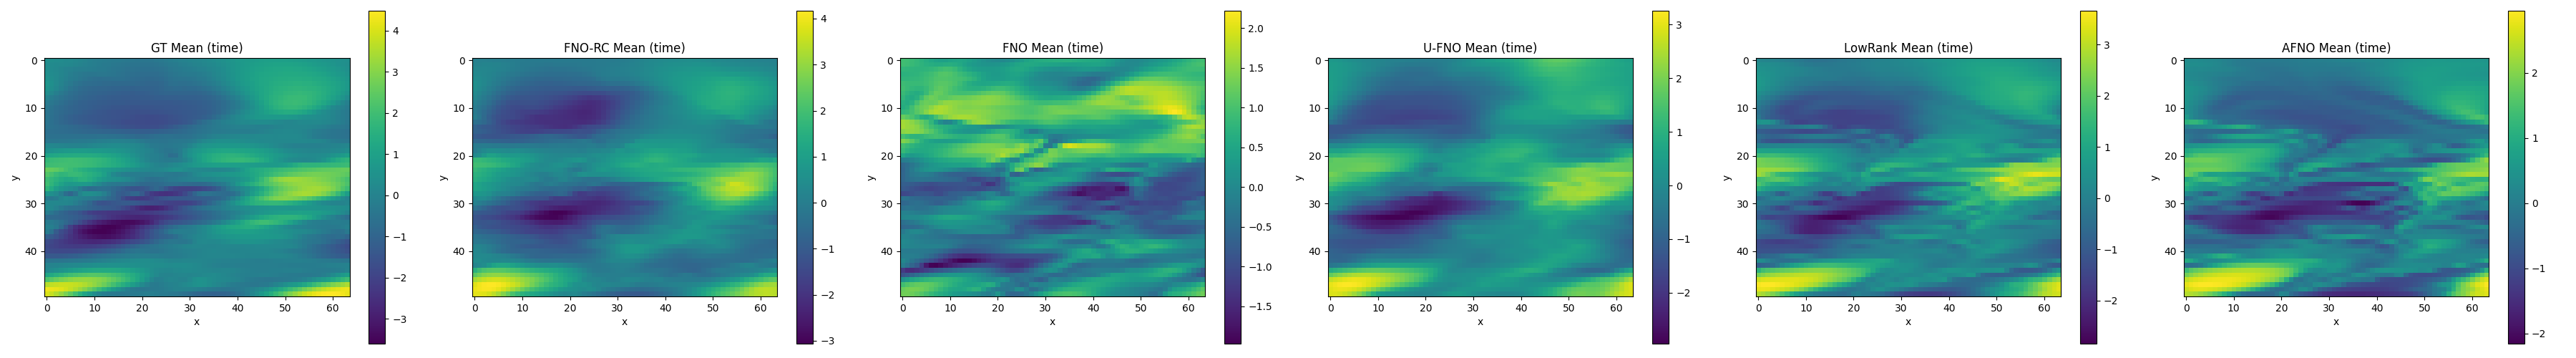
\includegraphics[width=\textwidth]{../实验图/mean_time.png}
    \caption{Time-averaged field: GT (left), FNO-RC (center), FNO (right). FNO-RC captures correct flow patterns with sharper features; FNO exhibits excessive diffusion.}
\end{subfigure}
\caption{\textbf{Qualitative 3D Navier-Stokes comparison.} FNO-RC faithfully renders fine structures, sharp gradients, and large-scale patterns. Reduced error accumulation evident in \textbf{(a)} instantaneous snapshots and \textbf{(b)} temporal averages.}
\label{fig:qualitative}
\end{figure}

\end{document}
